\documentclass[twocolumn]{article}
\usepackage{graphicx}
\usepackage{amsmath}
\usepackage{hyperref}
\usepackage{float}
\usepackage{geometry}

\geometry{top=2cm, bottom=2cm, left=3cm, right=2cm}

\begin{document}
\begin{titlepage}
    \centering
    \vspace*{1cm}
    
    {\LARGE \bfseries Department of Information and Communication Technology \par}

    \begin{figure}[H]
        \centering
        \includegraphics[width=0.75\linewidth]{logo.png}
        \label{fig:enter-label}
    \end{figure}
    
    \vspace{1cm}
    
    {\Huge \bfseries Machine Learning in Medicine \par}
    
    \vspace{1cm}
    
    {\Large Fetal Head Circumference Semantic Segmentation Report \par}
    
    \vfill
    
    \begin{minipage}{0.5\textwidth}
        \begin{flushleft}
            {\large \textbf{ID - Student Name:}} \\
            22BI13103 - Le Duc Dung - Data Science
        \end{flushleft}
    \end{minipage}%
    \begin{minipage}{0.5\textwidth}
        \begin{flushright}
            {\large \textbf{Lecturer:}} \\
            Prof. Tran Giang Son
        \end{flushright}
    \end{minipage}
    
    \vspace{2cm}
    
    {\large Academic year: 2022 - 2025} \par
    
    \vspace{1cm}
    
    {March 6, 2025}
    
\end{titlepage}

\begin{abstract}
The fetal head circumference (HC) is a useful tool to monitor gestational age in fetuses. I implemented a U-Net automation pipeline for computing the HC from 2D ultrasound images using annotation as patterns for model learning to perform a semantic segmentation task.
\end{abstract}

\section{Introduction}
To monitor gestational age and fetal growth, ultrasound imaging is used to measure fetal head circumference (HC). The HC18 challenge provides a dataset for automating HC computation from ultrasound images \cite{van2018automated}. After the lecture by Dr. Tran Giang Son, I decide to approach the HC18 challenge and build a U-net model to segment the fetal head masks and then compute to get results. The structure is as follows: \textnormal{filename, center\_x\_mm, center\_y\_mm, semi\_axes\_a, semi\_axes\_b, angle\_rad}.

\section{Methodology}
\subsection{Data Exploration}
The data set contains 1,343 two-dimensional (2D) ultrasound images of the standard fetus plane. The goal of the challenge is to automatically measure the HC in millimeters(mm) from these 2D ultrasound images. The data set is divided into 999 training images and 335 test images. Each image is 800 by 40 pixels, and the pixel sizes range between 0.052 and 0.326 mm. Additional information on pixel size per image is provided in the dataset. Training labels are included in the dataset as ellipses. The results should be submitted as a csv file with 6 columns and 336 rows.

\begin{figure}[H]
    \centering
    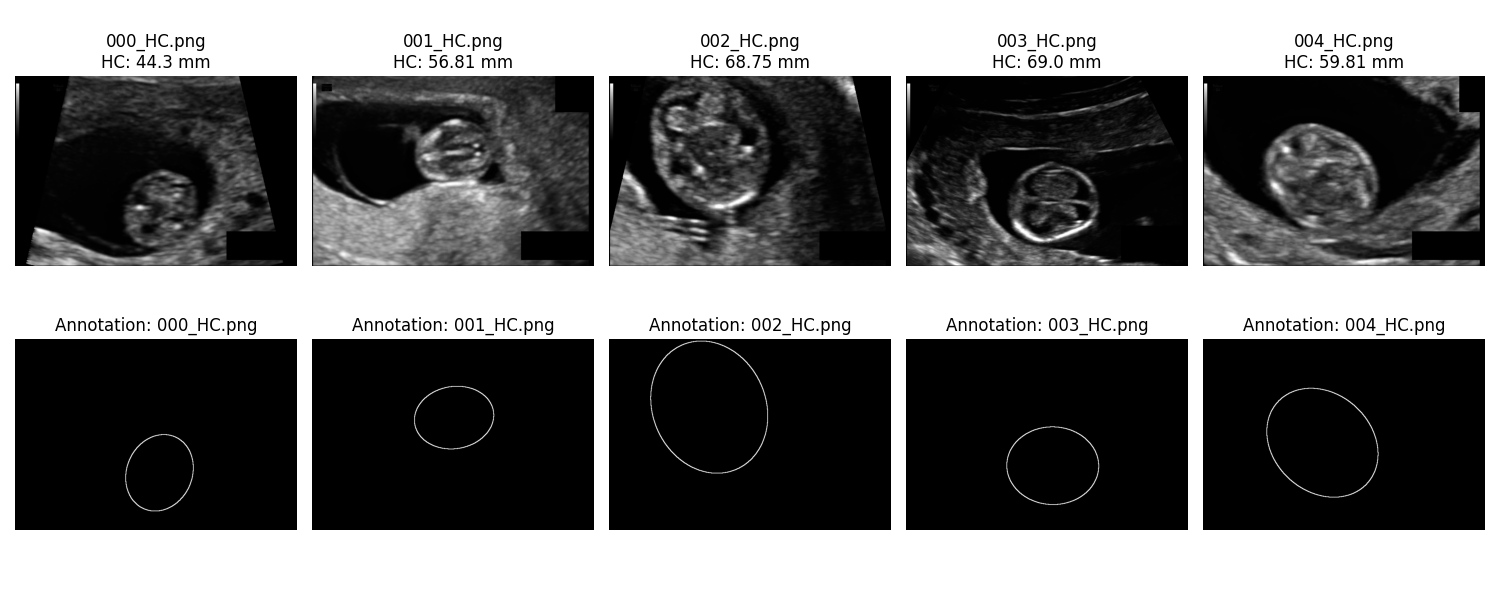
\includegraphics[width=1\linewidth]{figures/annotation_img.png}
    \caption{Training Images}
    \label{fig:enter-label}
\end{figure}

\subsection{Data Pre-processing}
The training labels were modified using OpenCV to fill in ellipses and stored in a separate directory as segmented masks. The training images were then normalized and resized to the input size.

\begin{figure}[H]
    \centering
    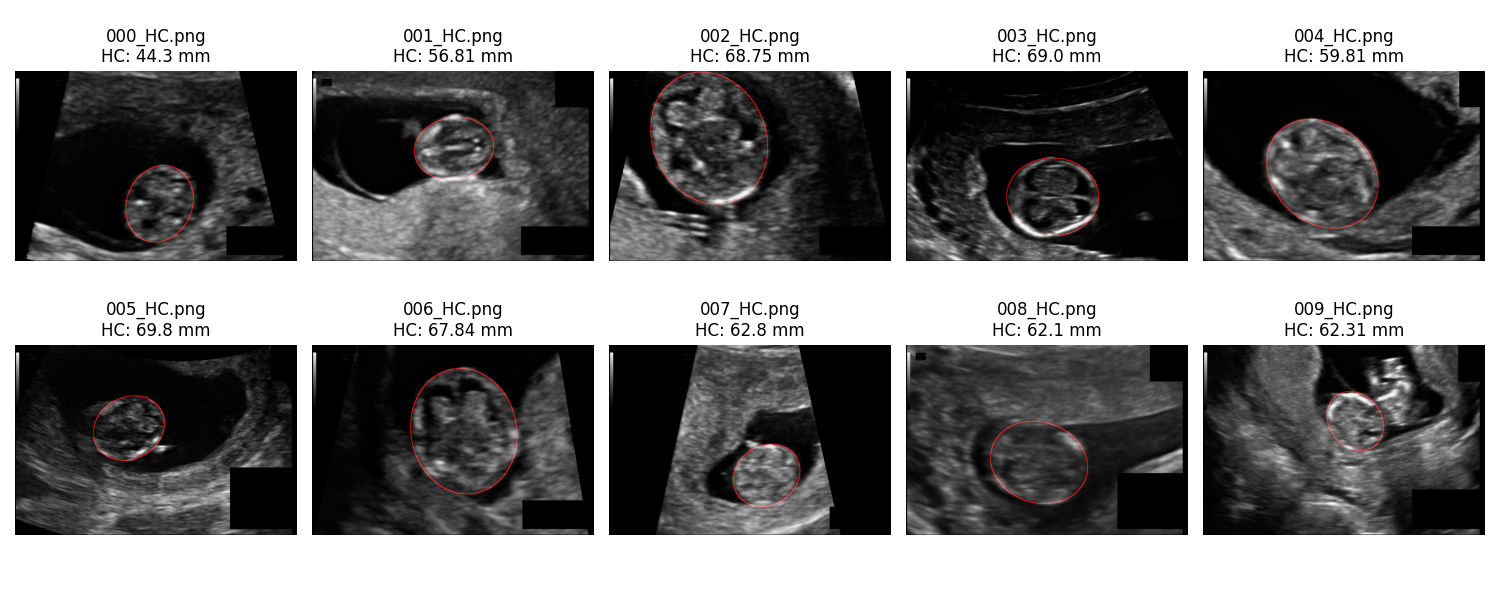
\includegraphics[width=1\linewidth]{figures/detect_border.png}
    \caption{Overlay annotation}
    \label{fig:enter-label}
\end{figure}

\begin{figure}[H]
    \centering
    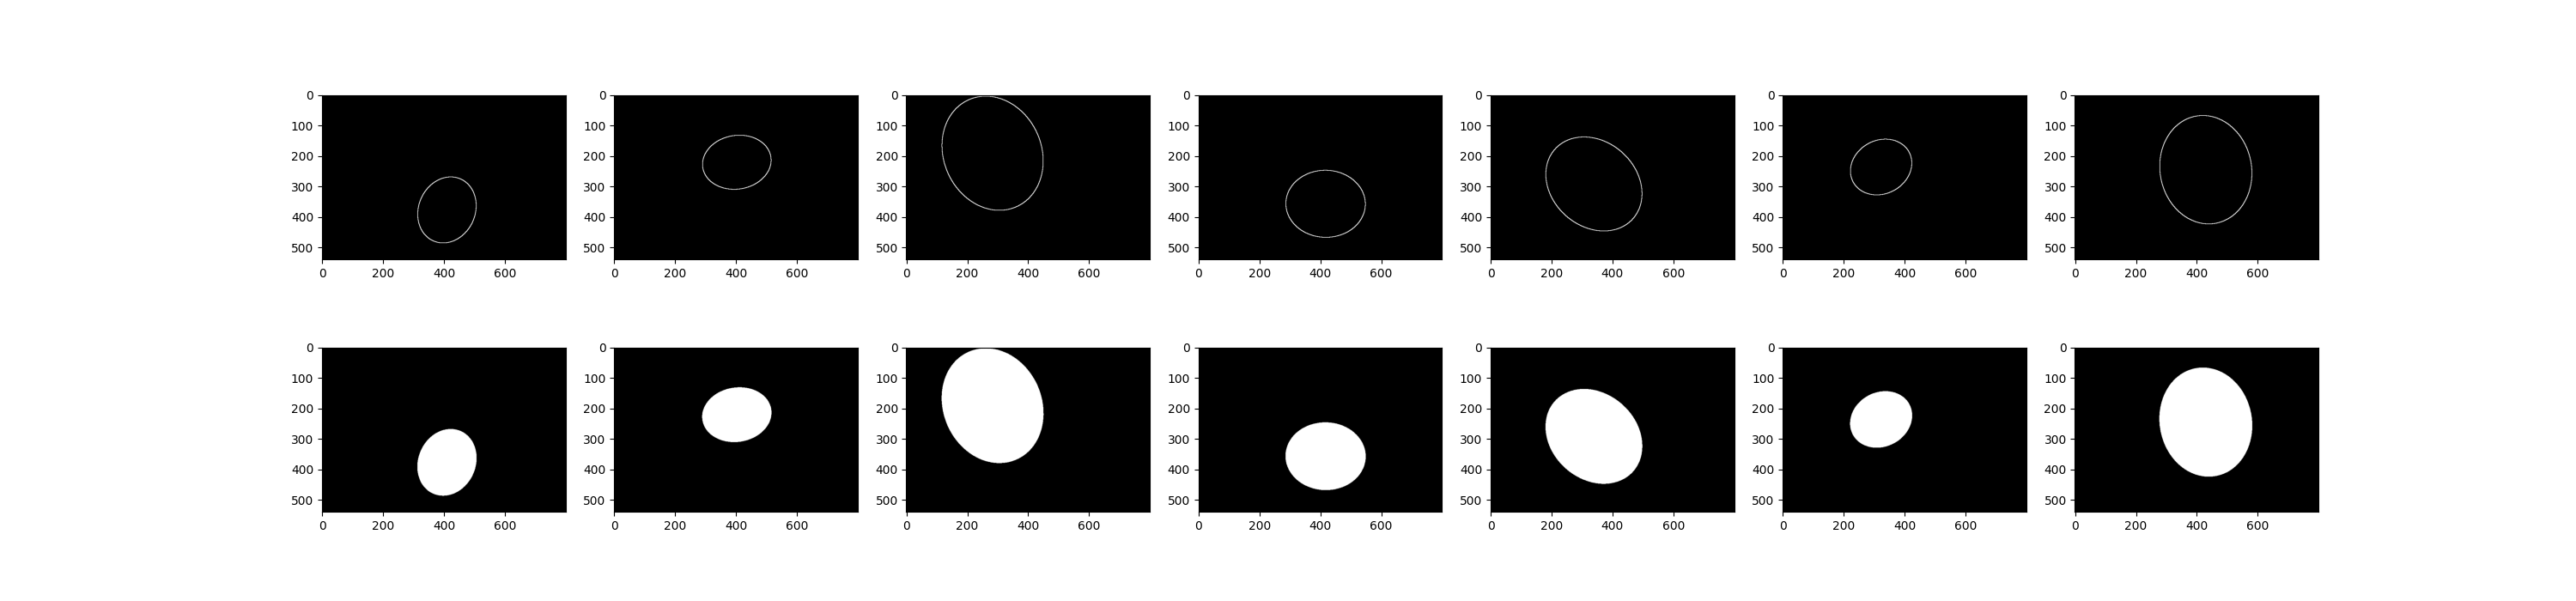
\includegraphics[width=1\linewidth]{figures/Fill-in Mask.png}
    \caption{Filled-in Masks}
    \label{fig:enter-label}
\end{figure}

\subsection{U-Net}
U-Net \cite{ronneberger2015u} was used for image segmentation. It consists of a contracting and expanding path. Adam optimizer with a learning rate of $1e^{-4}$ was used and dice loss was chosen. The model was built with tensorflow with encoder, bottleneck, and then the decoder part.

\begin{figure}
    \centering
    \includegraphics[width=1\linewidth]{image.png}
    \caption{U-Net Model Architecture}
    \label{fig:enter-label}
\end{figure}

\section{Implementation}
After data Pre-processing, I split the training set into traning set and validation set with ratio at 0.2 (80\% for training data and 20\% for validation data). I build model with three parts named encoder, bottleneck and decoder. The input is 256 by 256 pixels with one color channel, the encoder part contains \textbf{layers.Conv2D} with kernel size of 3 by 3 using ReLu as activate fuction then \textbf{layers.MaxPooling2D} to pool the convolutional layer. In the bottleneck, I apply 2 convolutional layers consecutively as the double convolutional layer. In the decoder part, I use \textbf{layers.Conv2DTranspose} as upsampling convolutional layers then concatenate it with symmetrically corresponding encoder feature maps. The output layer is applied sigmoid activate function because the ouput should be the mask of detected feature. In the training configuration, I set Adam as optimizer, dice loss as the loss function and Mean Absolute Error as metric for evaluation then I train U-net with 200 epochs, learning rate is 1e-4 and I set early stopping monitored by validation loss at patience 5 which mean the training process will stop if the validation loss does not improve in five consecutive epochs.

\section{Results}
U-Net achieved MAE score of 0.0102 as well as about 98,99\% of accuracy.
And model learned the patterns well with excellent performances that can be shown through the learning curves.

\begin{figure}[H]
    \centering
    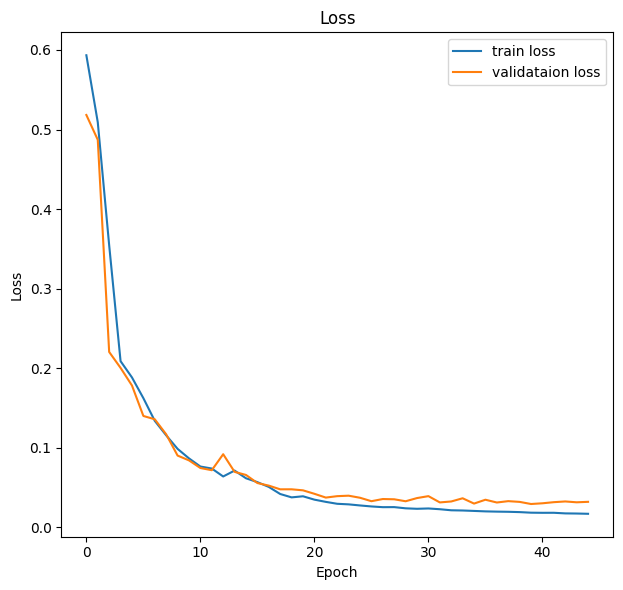
\includegraphics[width=1\linewidth]{figures/Loss_Learning_Curve.png}
    \caption{Loss Learning Curve}
    \label{fig:enter-label}
\end{figure}

When predicting U-net, the segment mask fits the original image well which is showing through mask overlay. 

\begin{figure}[H]
    \centering
    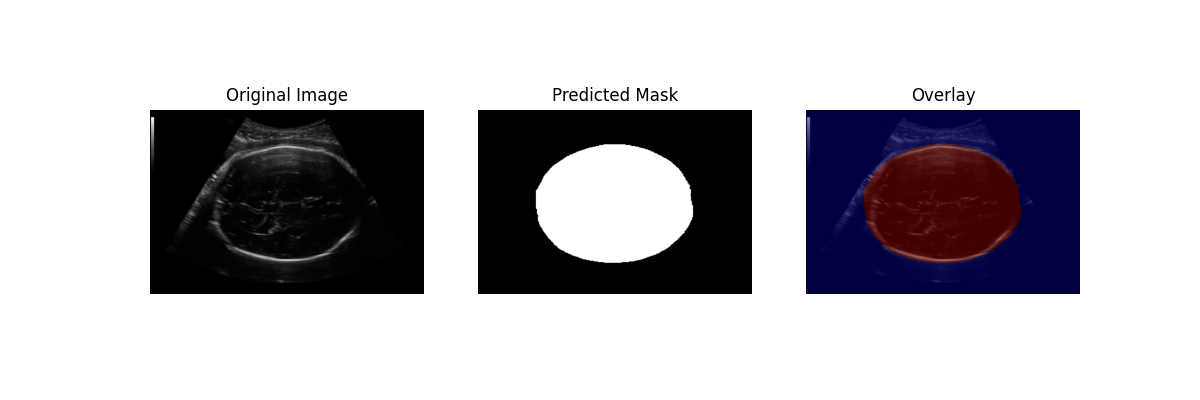
\includegraphics[width=1\linewidth]{figures/predicted_mask.png}
    \caption{Predicted Mask applying to 000\_HC.png}
    \label{fig:enter-label}
\end{figure}

\section{Conclusion}
I developed a pipeline for estimating fetal HC using U-Net build by Tensorflow. Future work can explore improved training of nnU-Net and alternative post-processing techniques.

\begin{thebibliography}{9}
\bibitem{van2018automated} Van den Heuvel et al., "Automated measurement of fetal head circumference using 2D ultrasound images," Zenodo, 2018.
\bibitem{ronneberger2015u} Ronneberger et al., "U-Net: Convolutional networks for biomedical image segmentation," arXiv preprint, 2015.
\end{thebibliography}

\end{document}
